%!TEX program = xelatex
\documentclass [a4paper]{article}
\author {SY1606407 王晓健}
\title {多元回归分析}
\date{}
\usepackage{ctex}
\usepackage{amsmath}
\usepackage{amssymb}
\usepackage{booktabs}
\usepackage{geometry}
\usepackage{graphicx}
\usepackage{multirow}
\geometry{left=2.5cm,right=2.5cm,top=2.5cm,bottom=2.5cm}
\begin{document}
\maketitle
\begin{abstract}
随着我国经济的迅速发展,人民生活水平不断提高,财政收入也不断上升,本文收集了北京市1995年-2014年年度各项经济指标数据,利用R语言进行多元回归分析,分析了地方财政收入与各项经济指标的关系,并对模型进行了统计检验和优化。
\end{abstract}

\begin{keywords}
关键词:多元线性回归,统计检验,逐步回归
\end{keywords}

\section{数据的收集与整理}
数据来源于《中国统计年鉴2015》中对北京市1995-2014年年度各项经济指标统计数据的查询结果,包含的统计项包括:地方财政一般预算收入(亿元)、地区生产总值(亿元)、	第一产业增加值(亿元)	、第二产业增加值(亿元)、	第三产业增加值(亿元)、	农林牧渔业增加值(亿元)、	工业增加值(亿元)、	建筑业增加值(亿元)、	金融业增加值(亿元)、	房地产业增加值(亿元)、	其他行业增加值(亿元)、	年末常住人口(万人)、	全社会固定资产投资(亿元)	房地产开发投资(亿元)、经营单位所在地出口总额(千美元)、	经营单位所在地进口总额(千美元),各项指标的基础统计结果如表1所示
\begin{table}[h]
\centering
\caption{各项指标的分布情况}
\small %此处写字体大小控制
\begin{tabular}{ccccc}
\toprule
指标&最小值&中位数&均值&最大值\\
\midrule
地方财政一般预算收入.亿元.&	115.3	&	 831.9	&	1370.6	&	4027.2\\
第一产业增加值.亿元.	&	72.16	&	 88.02&	101.61&	159.64\\
第二产业增加值.亿元.&	 645.8	&	1940.0&	2145.2&	4544.8\\
第三产业增加值.亿元.	&	789.7&	 4473.3	&	 6264.9&	6627.0\\
农林牧渔业增加值.亿元&	 72.16&	88.02&	01.83	&	161.83\\
工业增加值.亿元.	&	527.8	&	1630.9	&	1759.2&	3746.8\\
建筑业增加值.亿元.	&	18.0&	309.2	&	396.5	&	902.7\\
金融业增加值.亿元.	&	152.9&	777.0	&	1163.4&	3357.7\\
房地产业增加值.亿元.	&	 22.45	&	 464.92	&	579.23&	1339.52\\
其他行业增加值.亿元.	&	 289.1	&	2032.5	&	2855.4&	8110.2\\
年末常住人口.万人.	&	1248&	1516	&	618	&	2152\\
全社会固定资产投资.亿元.&	841.5	&	2677.7&	3179.5&	6924.2\\
房地产开发投资.亿元.	&	 328.2	&	1499.2&	1627.9	&	715.3\\
经营单位所在地进出口总额.千美元.&	29318330&	110041075	&	169260931	&	428995812\\
经营单位所在地出口总额.千美元.&	8119750	&	25717578&	32267436&	63097561\\
经营单位所在地进口总额.千美元.&	 19993150	&	 84323497&	136993494&	365898251\\
\bottomrule
\end{tabular}
\end{table}

\section{模型建立}
\subsection{多元线性回归方法简介}

回归分析是一种衡量因变量与自变量之间相关关系的统计分析方法。研究两个或两个以上自变量对因变量的回归分析方法称为多元回归分析,表现这一数量关系的数学公式被称为多元线性回归模型。设 $y$ 是随机变量,$x_1,x_2,...x_p$为 $p$ 个非随机变量,$\varepsilon$ 为随机误差,则 $y$ 与$x_1,x_2,...x_p$ 的多元线性回归模型表示为:
$$
y =\beta_0 +\beta_1x_1 +\beta_2x_2+....\beta_px_p +\varepsilon
$$
 其中 $\beta_0,\beta_1,...\beta_p$为 $p+1$ 个未知参数,称为回归系数,$y$ 称为被解释变量,$x_1,x_2,...x_p$称为解释变量,$\varepsilon$称为随机误差,一般假设$\varepsilon \sim \mathcal{N}(0,\sigma^2)$

在样本空间中选取 $n$ 个样本,若$y_i$与$x_{i1},x_{i2}...x_{ip}$ 存在多元线性相关关系,为了估计$\beta_0,\beta_1,...\beta_p$ ,可以建立以下方程组:
$$
\left\{
\begin{aligned}
y_1 = \beta_0+\beta_1x_{11}+\beta_2x_{12}+....+\beta_px_{1p}\\
y_2 = \beta_0+\beta_1x_{21}+\beta_2x_{22}+....+\beta_px_{2p}\\
.....\\
y_n = \beta_0+\beta_1x_{n1}+\beta_2x_{n2}+....+\beta_px_{np}\\
\end{aligned}
\right.
$$
该方程组可以写成矩阵的形式
$$
Y = X\beta +\varepsilon
$$
其中$Y=(y_1,y_2,...y_n)^T$ ,$\beta = (\beta_0,\beta_1,...\beta_p)^T$,$\varepsilon = (\epsilon_1,\epsilon_2,...\epsilon_n)$
$$
X = \begin{bmatrix}
1&x_{11}&x_{12}&...&x_{1p} \\
1&x_{21}&x_{22}&...&x_{2p} \\
.&.&.&...&.\\
.&.&.&...&.\\
1&x_{n1}&x_{n2}&...&x_{np} \\
\end{bmatrix}
$$
多元线性回归系数的求解一般使用最小二乘的方法,即找到向量$\beta = (\beta_0,\beta_1,...\beta_p)^T$,使得残差平方和 $Q=(Y-X\beta)^T(Y-X\beta)$ 最小,令$\frac{\partial Q(\beta)}{\partial \beta}=0$,得到
$$
\hat\beta = (X^TX)^{-1}X^TY
$$
经验回归方程为
$$
\hat y = \hat{\beta_0}+\hat{\beta_1}x_1+\hat{\beta_1}x_2+...++\hat{\beta_p}x_p
$$

\subsection{建立回归模型}

本文主要研究财政收入与各项指标之间的相关关系,设 $Y$ 为财政收入,$X$ 为解释变量$1,x_1,x_2,...x_{14}$ 组成的向量,分别表示第一产业增加值(亿元)	、第二产业增加值(亿元)、	第三产业增加值(亿元)、	农林牧渔业增加值(亿元)、	工业增加值(亿元)、	建筑业增加值(亿元)、	金融业增加值(亿元)、	房地产业增加值(亿元)、	其他行业增加值(亿元)、	年末常住人口(万人)、	全社会固定资产投资(亿元)	房地产开发投资(亿元)、经营单位所在地出口总额(千美元)、	经营单位所在地进口总额(千美元),$\beta$ 为未知参数向量,$\epsilon$ 为 $n$ 维随机误差向量,可以建立一个多元线性回归模型如下:
$$
Y=X\beta + \varepsilon
$$
使用R语言进行回归分析得到结果如表2所示
\begin{table}
  \centering
  \caption{回归分析参数结果}
  \small %此处
  \begin{tabular}{ccccc}
    \toprule
      解释变量名称 & 回归系数 & 估计标准差 & t值 & Pr(>|t|)  \\
    \midrule

    (Intercept)   & 2.097e+03 &   1.459e+03 &    1.437  &   0.2102 \\
    $x_1$: 第一产业增加值(亿元)      &      -2.527e+03  &  2.054e+03  &  -1.230  &   0.2733  \\
    $x_2$: 第二产业增加值(亿元)     &       5.350e+01  &  4.174e+01  &   1.282   &  0.2561  \\
    $x_3$: 第三产业增加值(亿元)      &      1.199e+00  &  5.086e-01  &   2.358   &  0.0649 \\
    $x_4$:  农林牧渔业增加值(亿元)       &     2.545e+03  &  2.060e+03  &   1.235  &   0.2716  \\
    $x_5$:  工业增加值(亿元)       &    -5.346e+01  &  4.152e+01  &  -1.288   &  0.2542  \\
    $x_6$: 建筑业增加值(亿元)      &     -5.463e+01  &  4.250e+01  &  -1.285   &  0.2550  \\
    $x_7$:   金融业增加值(亿元)     &     -2.078e+00  &  9.589e-01  &  -2.167  &   0.0824  \\
    $x_8$:   房地产业增加值(亿元)      &    -6.124e-01  &  4.609e-01  &  -1.329   &  0.2413  \\
    $x_9$:  其他行业增加值(亿元)      &    -6.465e-01  &  6.195e-01  &  -1.044   &  0.3445  \\
    $x_{10}$:   年末常住人口(万人)    &     -2.739e+00   & 1.553e+00  &  -1.764  &   0.1380  \\
    $x_{11}$:  全社会固定资产投资(亿元)     &     -3.792e-03  &  1.205e-01  &  -0.031   &  0.9761  \\
    $x_{12}$:  房地产开发投资(亿元)      &    -2.333e-01  &  2.010e-01  &  -1.161   &  0.2981  \\
    $x_{13}$:  经营单位所在地出口总额(千美元)   &    -3.838e-07  &  1.949e-06  &  -0.197   &  0.8516  \\
    $x_{14}$:  	经营单位所在地进口总额(千美元)        &     -3.356e-06   & 6.121e-06  &  -0.548   &  0.6071  \\
    \bottomrule

  \end{tabular}


\end{table}


\section{模型诊断和检验}

使用R语言建立回归模型如表2所示。

通过观察残差图可以从大体上对模型进行诊断:

1. 线性相关性检验:通过观察图1可以发现,残差分布均匀无规律,说明线性关系良好

2. 残差正态性检验:通过观察图2的Q-Q图可以发现,散点大致都集中在QQ图中的直线上,说明残差正态性良好。

3. 同方差检验:通过观察图3可以发现,残差在曲线周围均匀随机分布,可认为基本满足同方差假设

\begin{figure}[htbp]
  \centering
  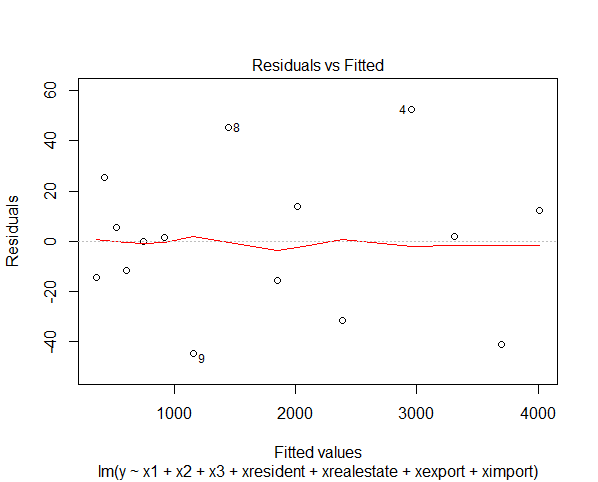
\includegraphics[width=0.35\textwidth]{img/Rplot.png}
  \caption{残差分布图}\label{fig:digit}
\end{figure}

\begin{figure}[htbp]
  \centering
  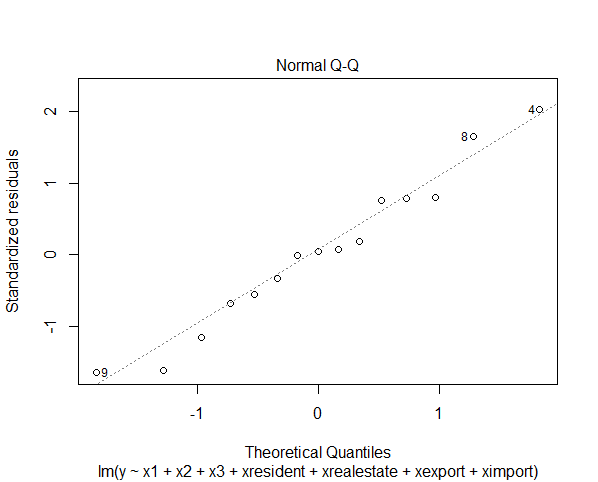
\includegraphics[width=0.35\textwidth]{img/Rplot02.png}
  \caption{残差QQ图}\label{fig:digit}
\end{figure}

\begin{figure}[htbp]
  \centering
  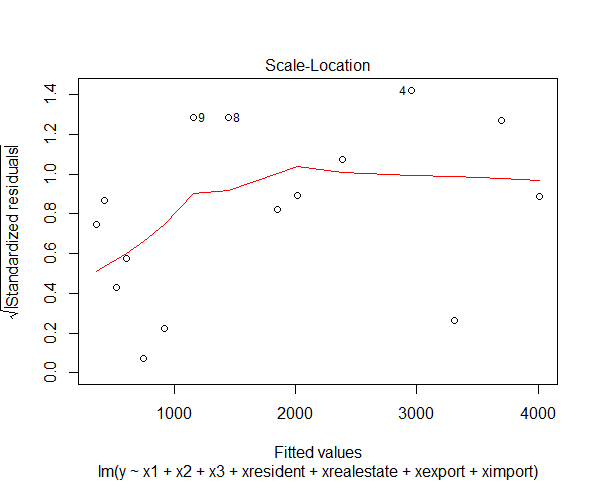
\includegraphics[width=0.35\textwidth]{img/Rplot03.png}
  \caption{标准化残差图}\label{fig:digit}
\end{figure}
\subsection{同方差检验}

所谓异方差性就是相对于不同的样本点,也就是相对于不同得解释变量观测值,随机误差项有不同的方差。检验异方差也就是检验随机误差项的方差与解释变量观测值之间的相关性,各种检验方法都是在这个思路下发展起来的。

在本文中我们使用 White 方法对模型进行异方差检验。White检验的基本思想是先用最小二乘法估计模型,将估计后的残差平方对常数项、解释变量、解释变量的平方和其交叉乘积等构成一个辅助回归,利用辅助回归建立相应的统计量来判断异方差性。

以二元线性回归为例,设模型为:
$$
y_i = \beta_0 +\beta_1x_{1i}+\beta_2x_{2i}+\varepsilon_i
$$
检验异方差性相当于假设检验问题:

$H_0:$ $\varepsilon_i$ 与解释变量不存在相关性 ,  $:H_1:$ ​ $\varepsilon_i$ 与解释变量存在相关性

White法可分为以下步骤:

1) 估计二元线性回归模型,并计算残差$\varepsilon_i$

2) 做如下辅助回归
$$
\varepsilon_i^2 = \alpha_0 +\alpha_1x_{1i}+\alpha_2x_{2i}+\alpha_3x_{1i}^2+\alpha_4x_{2i}^2+\alpha_5x_{1i}x_{2i}+\mu_i
$$
其中$\mu_i$为误差随机项

3) 计算统计量 $nR^2$ 的值,$n$为样本容量,$R^2$ 为辅助回归模型的可决系数

可以证明,在原假设成立的情况下,$nR^2 \sim \mathcal{X}^2(5)$,其中自由度5表示辅助回归模型中解释变量的个数

4) 给定显著性水平$\alpha$,查表得临界值$\mathcal{X}_\alpha^2(5)$,如果 $nR^2>\mathcal{X}_\alpha^2(5)$,则拒绝原假设$H_0$ ,表明随机变量存在异方差

使用White检验对模型进行异方差检验,得到chi2(166)    =    175.24,Prob > chi2  =    0.2965,p值比较大,则接受原假设,认为不存在异方差。
\subsection{残差正态性检验}


对多元线性回归进行统计检验的过程是建立在假设随机误差$\varepsilon_i$ 服从正态分布的基础之上的,一种常用的正态性检验是 Jarque-Bera 检验,简称 JB 检验,JB 检验中建立了 JB 统计量
$$
JB = \frac{n}{6}[S^2 + \frac{(K-3)^2}{4}]
$$
其中,$n$ 为样本容量,$S$ 为偏度系数,$K$ 为峰度系数,$S = \frac{\sum(x_i -\bar{x})^3}{n\sigma_x^3}$,用于衡量概率密度函数的对称性,$K=\frac{\sum(x_i-\bar{x})^4}{n\sigma_x^4}$,是对概率密度函数“胖瘦”的衡量,对于正态分布的总体,偏度为0,峰度为3,Jarque 和 Bera 证明了在正态假定下,$JB_{asy} \sim \mathcal{X}^2(2)$,给定显著性水平 $\alpha$ ,如果 JB 统计量的值超过了临界值 $\mathcal{X}^2_\alpha(2)$,则拒绝正态分布的假设。
使用R语言对回归的残差进行JB检验,得出JB = 0.35694, p-value = 0.809,p值很大,说明无法拒绝残差正态分布的假设。

\subsection{残差独立性检验}

在线性回归中,我们总是假设残差是彼此独立的(不相关)。如果违反相互独立假设 ,一些模型的拟合结果就会成问题。例如,误差项之间的正相关往往会放大系数 t 值,从而使预测变量显得重要 ,而事实上它们可能并不重要。

Durbin-Watson 统计量通过确定两个相邻误差项的相关性是否为零来检验回归残差是否存在自相关。该检验以误差均由一阶自回归过程生成的假设为基础。Durbin-Watson的检验统计量为:
$$
dw= \frac{\sum_{i=2}^n(\varepsilon_i-\varepsilon_{i-1})^2}{\sum_{i=1}^n\varepsilon_i^2}
$$


要从检验中得出结论,根据样本量n和自变量数目k'查DW分布表,得下临界值LD 和上临界值UD,并依下列准则判断残差的自相关情形:

(1)如果0<DW< LD ,则拒绝零假设,残差存在一阶正自相关。DW越接近于0,正自相关性越强。

(2)如果LD <DW< UD ,则无法判断是否有自相关。

(3)如果UD <DW<4-UD ,则接受零假设,残差不存在一阶正自相关。DW越接近2,判断无自相关性把握越大。

(4)如果4-UD <DW<4-LD ,则无法判断是否有自相关。

(5)如果4-LD <DW<4,则拒绝零假设,残差存在一阶负自相关。DW越接近于4,负自相关性越强。

使用R语言对模型进行Durbin-Watson检验,得到DW = 1.80, p-value = 0.1498,p值比较大,接受原假设,认为残差之间互相独立


\subsection{拟合优度检验}

在回归分析方法中,$y$ 与 $x_1,x_2...x_p$ 线性相关的密切程度可以用回归平方和 $U =\sum_{i=1}^{n}(\hat y_i -\bar y_i)^2$ 在总平方和 $L_{yy} = \sum_{i=1}^n (y_i - \bar y )^2$ 中所占的比例来衡量,即
$$
R^2= \frac{U}{L_{yy}}
$$
$R^2$ 称为拟合优度,$R^2$ 越接近于1,则称线性回归效果越显著。

使用R语言进行回归分析的结果显示,拟合优度$R^2 = 0.9999$ ,调整之后的拟合优度$R^2 = 0.9997$,说明回归方程拟合数据的程度很高。即根据当年的各类经济指标,可以非常准确地对财政收入作出估计。

\subsection{显著性检验}

在多元线性回归的方法中,显著性检验可以分为对回归方程的显著性检验和对回归系数的显著性检验。通常对回归方程的显著性检验使用F检验,对回归系数的显著性检验使用t检验。

\subsubsection{回归方程的显著性检验}

检验 $y$ 与 $x_1,x_2...x_p$ 之间有无线性关系实际上是假设检验问题:

$H_0:\beta_1= \beta_2 =...=\beta_p=0$ , $H_1:\beta_0,\beta_1,...\beta_p$ 不全为 0

设 $U = \sum_{i=1}^n(\hat y_i -\bar y)^2$, $Q=\sum_{i=1}^n(y_i-\hat y_i)^2$ ,可以证明 $U$ 与 $Q$ 相互独立,且
$$
\frac{Q}{\sigma^2} \sim \mathcal{X}^2(n-p-1)
$$
 在假设 $H_0$ 下,有
$$
\frac{U}{\sigma^2} \sim \mathcal{X}^2(p)
$$
因此可以建立F检验统计量
$$
\frac{(n-p-1)U}{pQ} \sim F(p,n-p-1)
$$
在给定水平 $\alpha$ 下,如果$F \ge F_{1-\alpha} (p,n-p-1)$,则拒绝原假设,认为被解释变量 $y$ 和解释变量之间存在线性相关关系

使用R语言对回归方程进行F检验,$F \sim F(p,n-p-1) \sim F(14,5)$,得到F值 =  3148, P值为6.832e-09,P值接近于0,说明回归方程有非常强的显著性。即财政收入和当年的各种经济指标之间存在很强的线性相关关系。
\subsubsection{回归系数的显著性检验}

对于每个解释变量 $x_i$ ,回归系数的显著性检验相当于假设检验问题:

$H_0: \beta_i=0$ ,$H_1:\beta_i \ne 0$

设矩阵$(X^TX)^{-1}$ 的主对角线元素依次为$c_{00},c_{11},...c_{pp}$,则$\hat \beta_i \sim N(\beta_i,c_{ii}\sigma^2)$ ,可以建立$t$ 统计量
$$
t_i =\frac{\hat \beta_i - \beta_i}{\hat \sigma \sqrt{c_{ii}}} \sim t(n-p-1)
$$
 当假设 0 成立时,可以建立检验统计量
$$
t_i = \frac{\hat \beta_i}{\hat \sigma \sqrt{c_{ii}}} \sim t(n-p-1)
$$
给定显著性水平 $\alpha $,若$|t_i| \ge t_{1-\frac{\alpha}{2}}(n-p-1)$,则拒绝原假设,认为变量 $x_i$ 对 $y$ 有显著的影响

使用R语言对回归系数进行t检验的结果如表1所示,可以发现对所有的解释变量,$P$ 值均大于 0.05,都没有通过显著性检验,即都不具有很强的显著性。但是回归方程的却很显著,这里猜测可能是解释变量之间存在较强的多重共线性导致的,这一点放在实际情况中也可以理解,因为各种经济指标之间往往是相互影响相互制约的。

\subsection{多重共线性检验}

模型中出现多重共线性将导致系数估计误差的增大,从而使 $t$ 统计量值减小,这就可能造成原来显著的值变成不显著。再统计学中,使用方差膨胀因子(VIF)来衡量最小二乘回归中多重共线性的严重程度,VIF衡量了回归系数的方差受到多重共线性的影响所增长的程度。VIF的计算分为三个步骤:

1) 对于每个解释变量 $x_i$,建立方程
$$
x_i = \sum_{j \ne i}^p \alpha_jx_j+c_0 +\varepsilon_{x_i}
$$
2) 计算每个解释变量 $x_i$ 的 VIF
$$
VIF = \frac{1}{1-R^2_i}
$$
其中 $R_i^2$ 是步骤一中方程的拟合优度

3)  如果 $0<VIF<10$,不存在多重共线性,$10 \le VIF \le 100$,存在较强的多重共线性,$VIF \ge 100$,存在严重的多重共线性

\section{模型优化}

\subsection{逐步回归}
由于在回归中,多个变量存在较为严重的多重共线性,在本文中,考虑采用逐步回归法对变量进行选择,逐步回归法的基本思想是逐个引入自变量,每次引入对 y 影响最显著的自变量,并对方程中的老变量进行逐个检验,把变得不显著的变量逐个从方程中剔除,最终的回归方程中既不漏掉对 y 影响显著的变量,也不包含对 y 影响不显著的变量。

其中前向逐步回归的步骤为:

1) 假设已经进行了$l$ 步筛选,并选入自变量$x_1,x_2...x_l$ ,现在进行第$l+1$ 步筛选,分别将自变量组 $(x_1,x_2,...x_l,x_{l+1}),(x_1,x_2,...x_l,x_{l+2}),(x_1,x_2,...x_l,x_{p})$ 与 $y$ 建立 $l+1$ 元回归方程,回归方程的F值分别为 ${F_{l+1}^{l+1},F_{l+2}^{l+1},...,F_p^{l+1}}$ ,记$F_{k_{l+1}}^{l+1} = \max\{ F_{l+1}^{l+1},F_{l+2}^{l+1},...,F_p^{l+1}\}$

2) 若 $F_{k_{l+1}}^{l+1} \le F_\alpha(1,n-(l+1)-1)$,则停止筛选,上一步得到的回归方程为最优方程

2) 若 $F_{k_{l+1}}^{l+1} \ge F_\alpha(1,n-(l+1)-1)$ ,则将 $x_{k_{l+1}}$ 选入模型,进行下一步筛选

在R语言中使用逐步回归的方法对变量进行剔除的结果如下所示:
Start:  AIC=133.49
y ~ x1 + x2 + x3 + x4 + x5 + x6 + x7 + x8 + x9 + x10 + x11 +
    x12 + x13 + x14

       Df Sum of Sq    RSS    AIC
- x11   1       0.7 3534.9 131.49
- x13   1      27.4 3561.6 131.65
- x14   1     212.5 3746.7 132.66
<none>              3534.2 133.49
- x9    1     769.8 4304.0 135.43
- x12   1     952.5 4486.7 136.26
- x1    1    1070.0 4604.2 136.78
- x4    1    1078.5 4612.8 136.82
- x2    1    1161.3 4695.5 137.17
- x6    1    1168.0 4702.2 137.20
- x5    1    1172.0 4706.2 137.22
- x8    1    1248.1 4782.3 137.54
- x10   1    2200.1 5734.3 141.17
- x7    1    3320.2 6854.4 144.74
- x3    1    3930.5 7464.7 146.44

Step:  AIC=131.49
y ~ x1 + x2 + x3 + x4 + x5 + x6 + x7 + x8 + x9 + x10 + x12 +
    x13 + x14

       Df Sum of Sq    RSS    AIC
- x13   1      41.6 3576.5 129.73
<none>              3534.9 131.49
- x14   1     449.1 3984.0 131.89
- x9    1     786.8 4321.7 133.51
- x12   1    1426.0 4960.9 136.27
- x1    1    1433.4 4968.3 136.30
- x4    1    1442.5 4977.4 136.34
- x2    1    1558.8 5093.7 136.80
- x5    1    1576.6 5111.5 136.87
- x6    1    1584.0 5119.0 136.90
- x8    1    1758.5 5293.4 137.57
- x10   1    2262.6 5797.5 139.39
- x7    1    3320.0 6854.9 142.74
- x3    1    3941.2 7476.1 144.47

Step:  AIC=129.73
y ~ x1 + x2 + x3 + x4 + x5 + x6 + x7 + x8 + x9 + x10 + x12 +
    x14

       Df Sum of Sq     RSS    AIC
<none>               3576.5 129.73
- x9    1     851.3  4427.9 132.00
- x12   1    1468.0  5044.5 134.61
- x1    1    2025.3  5601.8 136.70
- x4    1    2034.0  5610.5 136.73
- x2    1    2164.8  5741.3 137.19
- x6    1    2190.1  5766.6 137.28
- x5    1    2191.5  5768.0 137.29
- x14   1    2211.8  5788.3 137.36
- x10   1    2224.5  5801.1 137.40
- x7    1    3287.5  6864.0 140.77
- x3    1    3899.9  7476.4 142.48
- x8    1   11831.1 15407.6 156.94

可以看到在第一步中,删除了解释变量$x_{11}$,使得 AIC 值从 133.49下降到 131.49,
第二步中,删除了解释变量$x_{13}$,使得AIC值从 131.49 下降到 129.73,此后删除其余变量均不能使 AIC值降低,逐步回归结束。
\subsection{剔除变量增强回归系数的显著性}
对逐步回归后解释变量重新建立回归方程,得到的结果如表2 所示,可以发现删除了两个解释变量之后,其余变量的显著性虽然得到了一定的提高,但是大部分解释变量的回归系数仍然不够显著。因此考虑继续剔除变量使得回归系数显著。方法是每次选择剔除之后使得AIC增加最小的变量,直到再次剔除任何一个变量都会使AIC上升较为明显时停止。
根据这一方法,又依次剔除了解释变量$x_{9}$,$x_{12}$,$x_{14}$,$x_1$,$x_6$,每次剔除之后AIC值的变化如表3所示。
\begin{table}
  \caption{根据AIC剔除变量}
  \label{}
  \tiny
  \centering
  \begin{tabular}{cccccccccccccc}
    \toprule
    &none&$x_1$&$x_2$&$x_3$&$x_4$&$x_5$&$x_6$&$x_7$&$x_8$&$x_9$&$x_{10}$&$x_{12}$&$x_{14}$\\
    \midrule
    第一步&129.73&136.70&137.19&142.48&136.73&137.29&140.77&137.28&140.77&132.00&137.40&134.61&137.36\\
    第二步&132.00&136.42&137.26&166.25&136.47&137.41&137.05&145.97&155.56&&140.67&132.61&135.70\\
    第三步&132.61&134.72&135.49&166.84&134.76&135.63&135.27&144.36&155.37&&145.62&&133.71\\
    第四步&135.71&135.34&135.98&166.40&135.39&136.10&135.62&143.02&155.68&&146.06&&\\
    第五步&134.52&&149.18&165.94&144.96&153.18&&144.68&152.83&&152.41\\

    \bottomrule
  \end{tabular}

\end{table}

得到模型的回归结果如表4所示。可以看到各个回归系数的显著性都很高。最后得到的回归方程为
$$y = 1512.60481 +1.60768x_2 +0.46376x_3+6.48722x_4 -1.91999x_5 -0.57672x_7 -0.51914x_8 - 1.73536x_{10}$$
其中解释变量 $x_5$,$x_7$,$x_8$,$x_{10}$ 的回归系数为负数,事实上财政收入跟这些因素都是正相关的,这说明逐步回归之后并不能完全消除多重共线性的影响,但是其在保证模型精度的基础上尽可能简化了模型,使得使用比较少的解释变量就能准确地对因变量进行预测,其意义仍是积极的。
\begin{table}
  \centering
  \caption{回归分析参数结果}
  \small %此处
  \begin{tabular}{ccccc}
    \toprule
      解释变量名称 & 回归系数 & 估计标准差 & t值 & Pr(>|t|)  \\
    \midrule
    (Intercept) &1512.60481  &471.13758 &  3.211 &0.007485 \\
    $x_2$: 第二产业增加值(亿元) &  1.60768   &   0.40705   &  3.950  & 0.001929 \\
$x_3$: 第三产业增加值(亿元)      &     0.46376  &      0.06443 &  7.198  &   1.09e-05 \\
$x_4$:  农林牧渔业增加值(亿元)      &         6.48722  &  2.01709   &3.216& 0.007407 \\
$x_5$:  工业增加值(亿元)   &         -1.91999   & 0.41205  &-4.660& 0.000551 \\
$x_7$:   金融业增加值(亿元)   &         -0.57672    &0.18207  &-3.168& 0.008107 \\
$x_8$:   房地产业增加值(亿元)  &      -0.51914 &   0.11296 & -4.596& 0.000616 \\
$x_{10}$:   年末常住人口(万人) &        -1.73536  &  0.38391 & -4.520& 0.000702 \\

    \bottomrule

  \end{tabular}


\end{table}
\end{document}
